\section {BLE node}
\label {Impl_BLEnodeSection}

The sensing node is supposed to be installed on the container. For the demonstration purposes, we used a Raspberry Pi 3 device running NodeJs.

The BLE node has a DHT22 sensor that is able to sense temperature and humidity. The following diagram shows the wiring setup between the Raspberry device and the sensor. The sensor has 3 pin connections - 2 of them being used for power (VCC and ground) while the third is for transferring data. The a compatible driver for this sensor is required to be installed on the node.

\bigskip
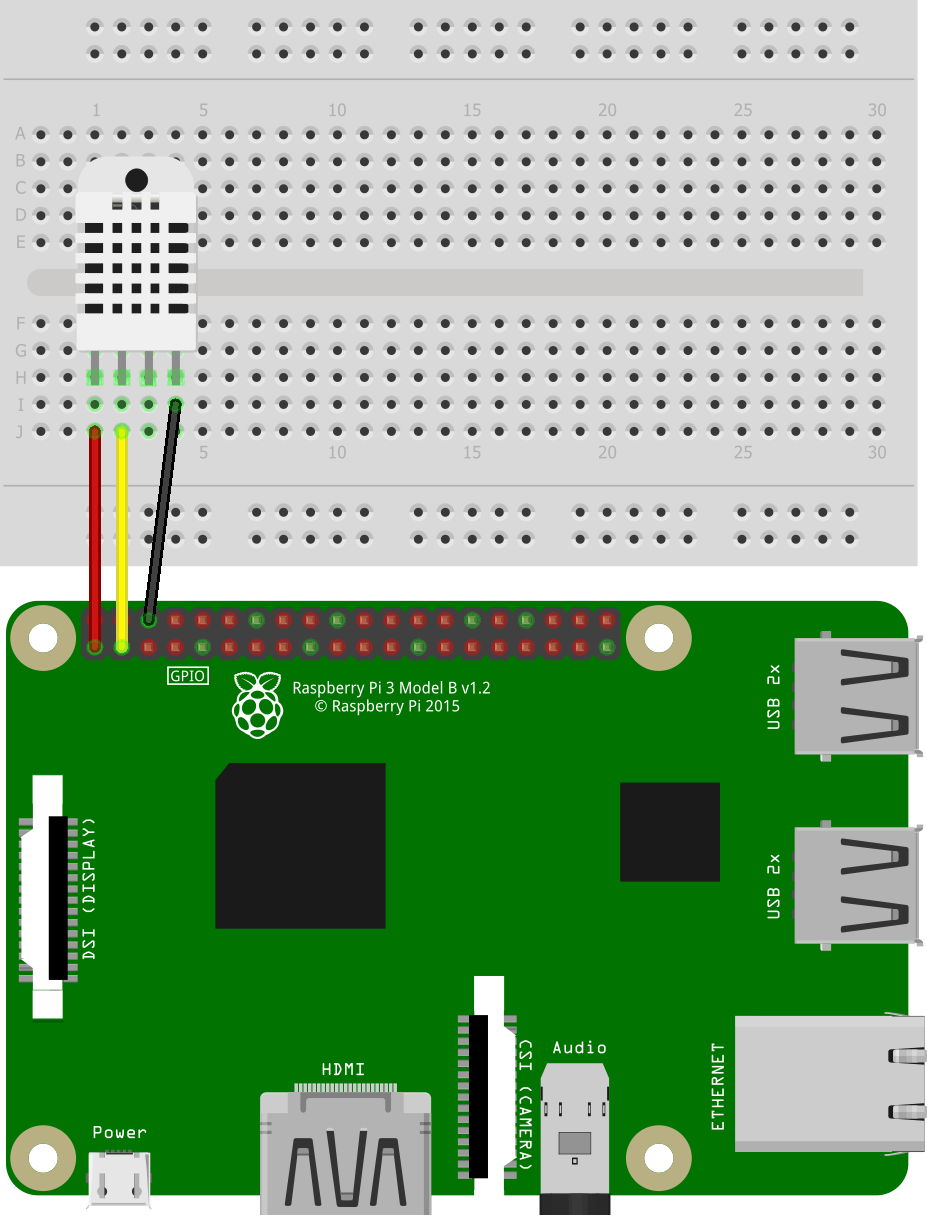
\includegraphics[scale=0.7]{gfx/RaspberrySensorNode} 
\bigskip

To interface with the sensor from the Node application, a npm package called node-dht-sensor needed to be added to the project.

The Nodejs application for the BLE node is structured as shown in the following diagram. For each of the components, the most important public methods are shown in order to show the interfacing between them. Private methods and members are not included to maintain the simplicity of the diagram.

\bigskip
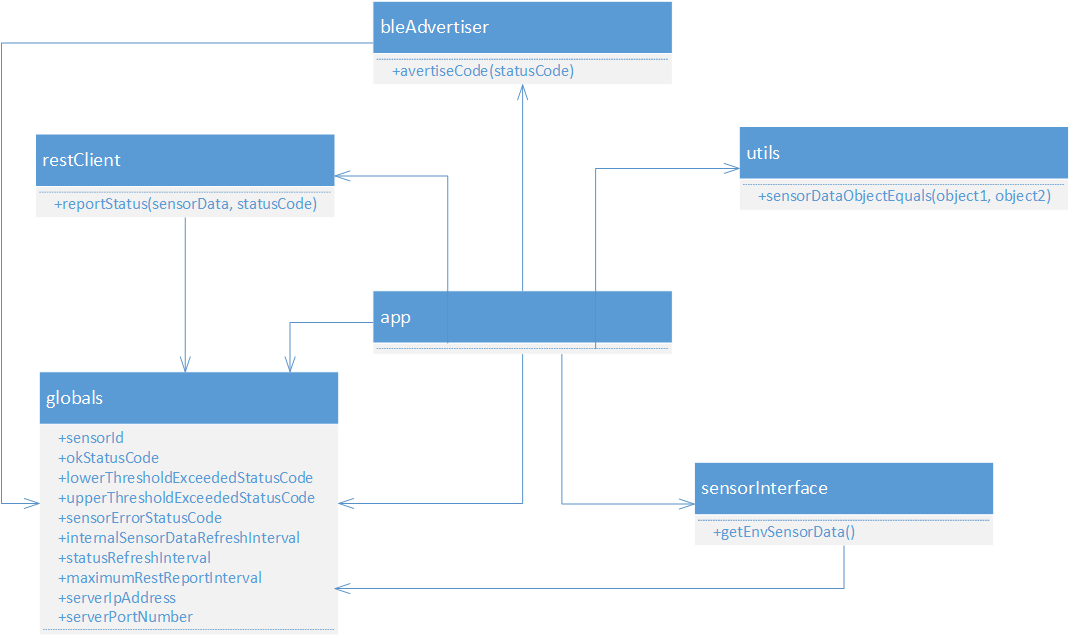
\includegraphics[scale=0.6]{gfx/bleNode_architecture} 
\bigskip

For each file, a short description of its purpose is provided.
\begin{itemize}
\item bleAdvertiser - class used for handling the BLE broadcasting. The sensor id and status code are broadcasted as the name of the device, separated by a semi-column. As the maximum name size allowed is 31 bytes, this field is more than enough for the information we require to make public. The class has only one public method that takes as argument the status code to broadcast.
\item restClient - class incorporating the logic and callbacks for making rest API calls over the network. This class exposes one public method used by the application to report the status and sensor data to the main server.
\item sensorInterface - class constantly pooling the data from the sensor and providing it when needed to the main application logic. This class is using an internal timer to control the frequency of poling sensor data.
\item utils - class containing helper methods used by the other components in the application. In this class, one method for comparing two different instances of sensor data in json format is provided. This is required to prevent the node from sending redundant data to the main server.
\item app - this is the main class of the application. It incorporates the rules and conditions for determining the status codes and uses most of the other classes, each having a specific role.
\item globals - class used for holding a set of global variables used throughout the application. The containing json file can therefore be used as application configuration that has different contents depending on the deployment sensor nodes.
\end{itemize}

The BLE node is designed to call only one REST method on the main server - reportStatus. This has been however thought so the sensor can both report data and aliveness. The sensor therefore calls the method each time the data or sensor status changes. If the measured values are constant, a call will be made every minute. This ensures that the time interval between 2 sensor updates is 60 seconds or less. Using this approach allows the server to determine whether the sensor is no longer active/connected to the network and inform the users accordingly. 



